\chapter{ Analyse et Sp\'{e}cifications des besoins }
\section{Introduction}


Cette partie consiste en une \'{e}tape analytique dans laquelle nous allons
recenser et factoriser les besoins des utilisateurs de l'application. Ceci est
fortement li\'{e} \`{a} l'\'{e}tude du projet men\'{e}e au
Cours du premier chapitre.
Pour ce faire cette phase doit r\'{e}pondre aux questions suivantes :
Quels sont les besoins fonctionnels de l'application ?
Quelles sont les contraintes qui doivent \^{e}tre prises en consid\'{e}ration?

   \section{ Les acteurs du syst\`{e}me }
C'est une entit\'{e} externe qui agit sur le syst\`{e}me (op\'{e}rateur, autre syst\`{e}me,
\ldots{}).Il peut consulter
Ou modifier l'\'{e}tat du syst\`{e}me.
En r\'{e}ponse \`{a} l'action d'un acteur, le syst\`{e}me fournit un service qui
correspond \`{a} son besoin.
Le principal acteur de syst\`{e}me :
\begin{itemize}
\item{  \textbf{L'administrateur :} entit\'{e} externe principale. Son r\^{o}le est qui a le droit de
g\'{e}rer un projet (cr\'{e}er, modifier, supprimer).
Aussi son r\^{o}le et de g\'{e}rer l'affectation des taches aux membres
correspondants.
}

\item{ \textbf{Le membre : } entit\'{e} externe secondaire, il peut se connecter pour consulter la
t\^{a}che en cours que l'administrateur lui a effectu\'{e} et la marquer comme
termin\'{e}e ou non.
}
\end{itemize}

La Table 2.1 pr\'{e}sente les roles selon les acteurs.

\begin{table}[H]
\centering
\begin{tabular}{|l|l|l|}
\hline
                                            & Administrateur & Membre  \\
\hline
Authentification~                           & X              & X       \\
\hline
Création d’un projet                        & X              &         \\
\hline
Ajout d’une tache                           & X              & X       \\
\hline
Modifier l’état d’une tâche                 & X              &         \\
\hline
Ajout d’un client/membre                    & X              &         \\
\hline
Consultation des rapports                   & X              &         \\
\hline
Consulter la carte géographique des clients & X              & X       \\
\hline
\end{tabular}
\centering
\caption{Rôles  des acteurs.}
\end{table}


\section{ Sp\'{e}cifications des besoins}

  \subsection{Besoins fonctionnels}

Le besoin primordiale de notre application et de permettre à l’administrateur
de « Cherchini » de gérer les projets et ceci consiste à :

\subsubsection{G\'{e}rer les projets}

\begin{itemize}
\item{La cr\'{e}ation d’un projet.}
\item{La modification d'un projet.}
\item{La suppression d'un projet.}
\item{La consultation des projets et des t\^{a}che et leurs d\'{e}tails correspondants.}
\item{L'affectation des membres correspondants \`{a} chaque projet.}
\end{itemize}

\subsubsection{G\'{e}rer les t\^{a}ches}

\begin{itemize}
\item{La cr\'{e}ation d'une t\^{a}che.}
\item{La modification d'une t\^{a}che.}
\item{La suppression d'une t\^{a}che.}
\item{La consultation  des t\^{a}che et des d\'{e}tails correspondants.}
\item{L'affectation du membre correspondant \`{a} chaque t\^{a}che.}
\end{itemize}

\subsubsection{G\'{e}rer les membres}

\begin{itemize}
\item{La cr\'{e}ation d'un membre.}
\item{La modification d'un membre.}
\item{La suppression d'un membre.}
\item{La consultation des membres et de leurs d\'{e}tails correspondants.}

\end{itemize}

\subsubsection{G\'{e}rer les clients}

\begin{itemize}
\item{La cr\'{e}ation d'un client.}
\item{La modification d'un client.}
\item{La suppression d'un client.}
\item{La consultation des clients et leurs d\'{e}tails correspondants.}
\end{itemize}

\subsubsection{
Suivre le d\'{e}roulement des projets}

\begin{itemize}
\item{ La suivie du travail en consultant le diagramme Gantt pour chaque projet.}
\item{La consultation des rapports des co\^{u}ts et les dur\'{e}es selon les projets et les clients   .}
\item{La consultation de la carte g\'{e}ographique des g\'{e}olocalisations des  clients.}
\end{itemize}

  \subsection{Besoins non fonctionnels}
Les besoins non fonctionnels sp\'{e}cifient les propri\'{e}t\'{e}s du syst\`{e}me afin de
garantir la Coh\'{e}rence, la confidentialit\'{e} et l'int\'{e}grit\'{e} des donn\'{e}es.
Le syst\`{e}me doit \^{e}tre fiable: la validit\'{e} de l`application.
R\'{e}utilisabilit\'{e}: aptitude de site \`{a} \^{e}tre utilis\'{e} en tout ou en partie dans de
nouvelles applications.

\subsubsection{La performance d'ex\'{e}cution}

Le temps d'ex\'{e}cution du syst\`{e}me doit \^{e}tre minimal pour ne pas g\^{e}ner
l'utilisateur. Ce temps d\'{e}pend de la complexit\'{e} du code impl\'{e}ment\'{e}, du
serveur d'application utilis\'{e}, du d\'{e}bit de la ligne de connexion et de la
conception de la base de donn\'{e}es.

\subsubsection{La s\'{e}curit\'{e}}

Le syst\`{e}me doit respecter un niveau de s\'{e}curit\'{e} \'{e}lev\'{e} afin de garantir la
confidentialit\'{e} de l'acc\`{e}s des membres

\subsubsection{L'ergonomie }

L'interface de cette application doit \^{e}tre ergonome, conviviale et voire m\^{e}me
apte \`{a} aider l'utilisateur \`{a} mieux g\'{e}rer son espace de travail.


\section{ Diagramme de cas d'utilisation g\'{e}n\'{e}rale }
Le diagramme de cas d'utilisation permet de d\'{e}crire l'interaction entre
l'acteur et le syst\`{e}me.
Le cas d'utilisation est une description des interactions qui vont permettre \`{a}
l'acteur d'atteindre son objectif en utilisant le syst\`{e}me. Un acteur et un cas
d'utilisation sont mis en relation par une association repr\'{e}sent\'{e}e par une
ligne.
Le but principal du diagramme du cas d'utilisation est de d\'{e}finir le syst\`{e}me
du point de vue des utilisateurs et de d\'{e}finir les limites pr\'{e}cises du syst\`{e}me en
utilisant une notation tr\`{e}s simple






\FloatBarrier
\begin{figure}[H]
\center
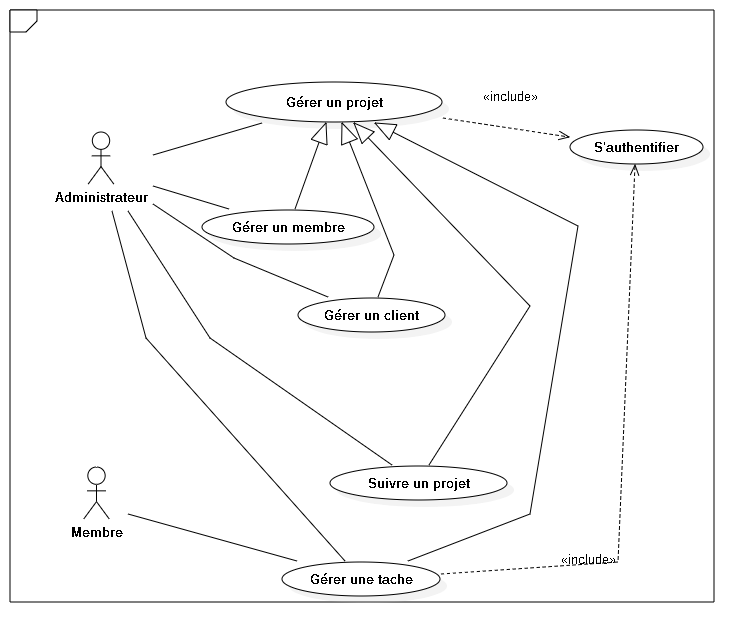
\includegraphics[width=13cm,height=10cm]{./figures/ucG.png}
\caption{Diagramme de cas d'utilisation g\'{e}n\'{e}rale.}

\end{figure}
\FloatBarrier




\section{Backlog de produit}

Apr\'{e}s avoir d\'{e}finit les acteurs des systémes et les diff\'{e}rentes interactions nous pouvons maintenant définir notre Product Backlog
puis nous pr\'{e}cisions la planification des sprints.

\subsection{Les fonctionnalit\'{e}s du Backlog}
Le Backlog est un art\'{e}fact tr\`{e}s important dans SCRUM. C'est l'ensemble des caract\'{e}ristiques
fonctionnelles ou techniques qui constituent le produit souhait\'{e}.
Nous allons les d\'{e}crire en d\'{e}tails dans le tableau qui suit :



\begin{table}

\begin{tabular}{|l|l|l|}
\hline
Fonctionnalité                                                                                              & Acteur                          & Description                                                                                                                                                     \\
\hline
Gérer un projet                                                                                             & Administrateur                  & \begin{tabular}[c]{@{}l@{}}L’administrateur peut gérer un projet et ses \\tâches correspondantes d’affectation\end{tabular}                                     \\
\hline
Mettre à jour un                                                                                            & \multirow{3}{*}{Administrateur} & \multirow{3}{*}{\begin{tabular}[c]{@{}l@{}}L’administrateur peut changer les détails \\du projet ainsi que l’affectation des membres\\~au projet\end{tabular}}  \\
\cline{1-1}
Projet                                                                                                      &                                 &                                                                                                                                                                 \\
\cline{1-1}
                                                                                                            &                                 &                                                                                                                                                                 \\
\hline
\begin{tabular}[c]{@{}l@{}}Créer ,Modifier ,\\Supprimer un membre\end{tabular}                              & Administrateur                  & \begin{tabular}[c]{@{}l@{}}L’administrateur peut manipuler les données \\des membres\end{tabular}                                                               \\
\hline
\begin{tabular}[c]{@{}l@{}}Créer ,Modifier ,\\Supprimer un client\end{tabular}                              & Administrateur                  & \begin{tabular}[c]{@{}l@{}}L’administrateur peut manipuler les \\données des clients\end{tabular}                                                               \\
\hline
Consulter les rapports                                                                                      & Administrateur                  & L’administrateur peut accéder aux rapports                                                                                                                      \\
\hline
\begin{tabular}[c]{@{}l@{}}Consulter les coordonnées \\des clients sur la carte\\~géographique\end{tabular} & Administrateur                  & \begin{tabular}[c]{@{}l@{}}L’administrateur peut accéder aux \\coordonnées géographiques des clients\end{tabular}                                               \\
\hline
\begin{tabular}[c]{@{}l@{}}Changer l’état et la\\~progression approximative \\de ses tâches\end{tabular}    & Membre                          & \begin{tabular}[c]{@{}l@{}}Le membre peut changer ses taches \\courantes selon l’avancement.\end{tabular}                                                       \\
\hline
\end{tabular}
\centering
\caption{Product Backlog}
\end{table}

\newpage

\subsection{ Planification des sprints}

\FloatBarrier
\begin{table}

\begin{tabular}{|l|l|l|}
\hline
\multirow{2}{*}{Release 1} & Gestion des projets                        & 20 jours  \\
\cline{2-3}
                           & Gestion des membres                        & 7 jours   \\
\hline
\multirow{5}{*}{Release 2} & Gestion des clients                        & 2 jours   \\
\cline{2-3}
                           & Authentification                           & 5 jours   \\
\cline{2-3}
                           & Création des interfaces administrateurs    & 20 jours  \\
\cline{2-3}
                           & Création des interfaces membres            & 5 jours   \\
\cline{2-3}
                           & Modification et design des interfaces~ ~ ~ & 15 jours  \\
\hline
\multirow{2}{*}{Release 3} & Intégration des données                    & 10 jours  \\
\cline{2-3}
                           & Affichage des rapports                     & 7 jours   \\
\hline

\end{tabular}
\centering
\caption{Planification des sprints }
\end{table}
\FloatBarrier


\subsection{Diagramme de Gantt}

\FloatBarrier
\begin{figure}[H]
\center
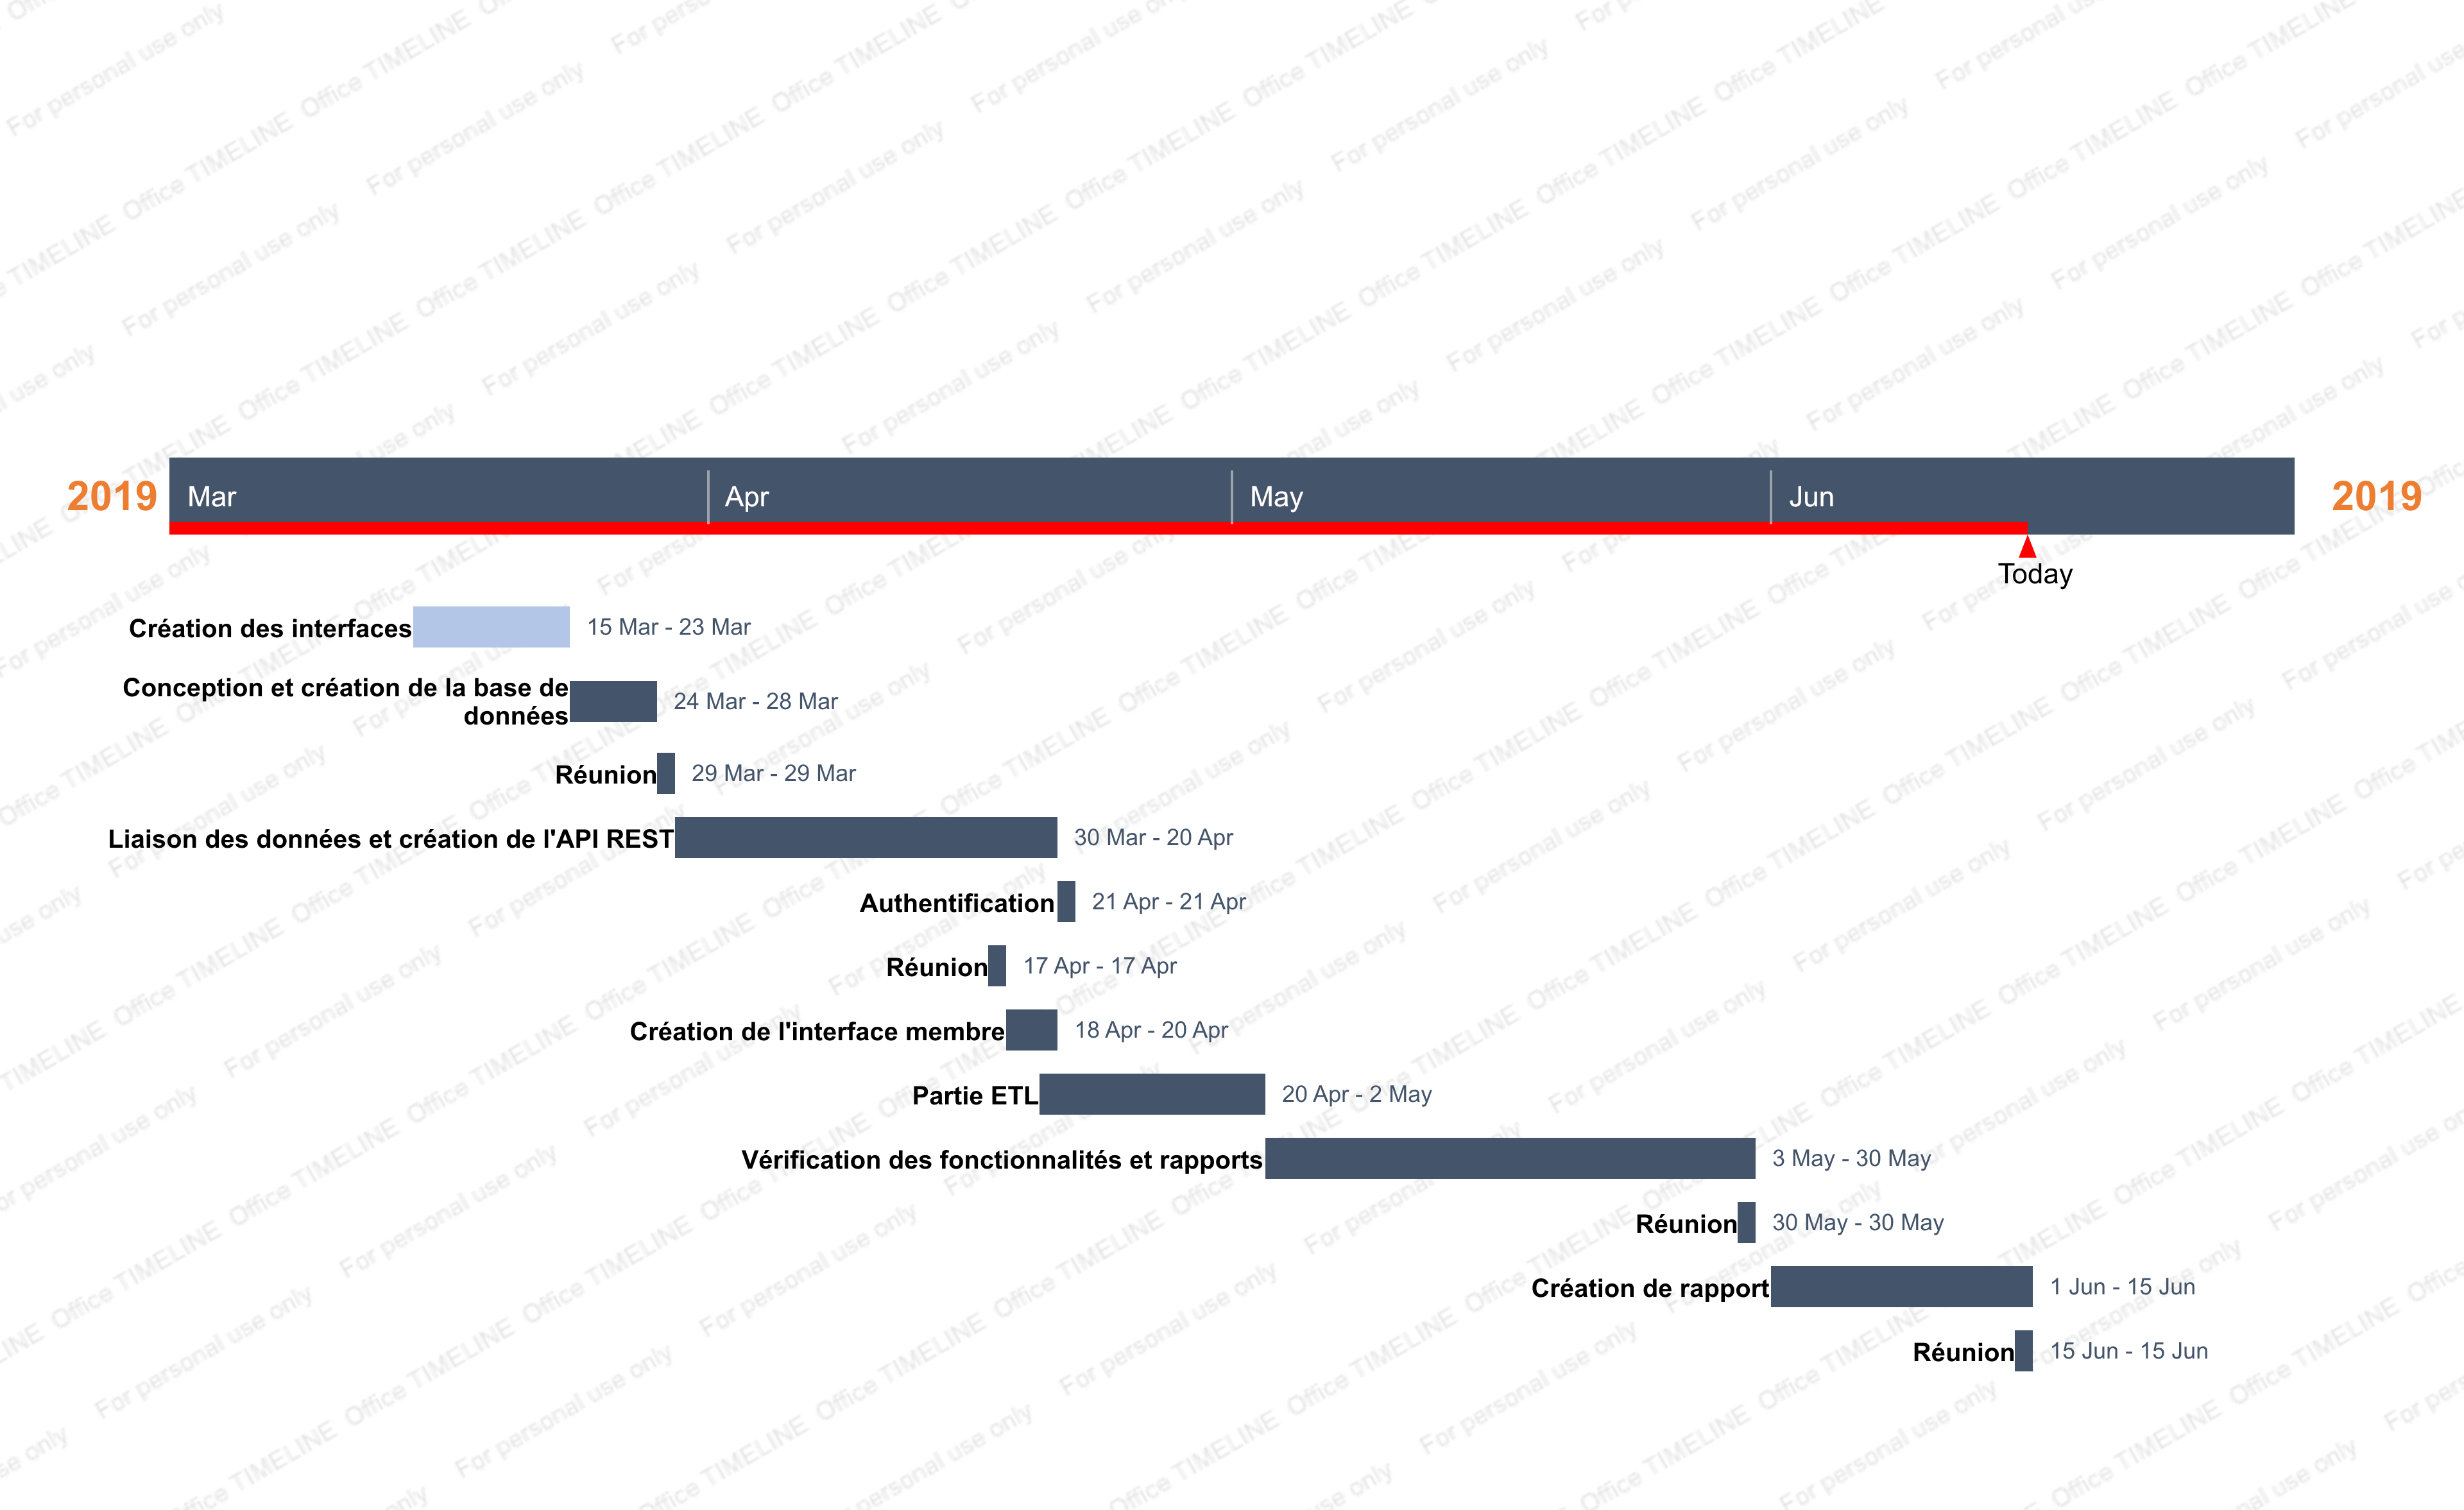
\includegraphics[width=15cm,height=15cm]{./figures/gantt.png}
\caption{Diagramme de Gantt.}
\end {figure}
\FloatBarrier


\section{Architecture de l application}
\subsection{Impl\'{e}mentation et structure}
Enfin nous d\'{e}crivons les \'{e}tapes globales suivies lors de la r\'{e}alisation de ce projet.
Les \'{e}tapes \'{e}taient :
\bigskip


\textbullet{}  Cr\'{e}er le site web statique (front -end)  \newline
\textbullet{} Cr\'{e}er une application express js  \newline
\textbullet{}  Cr\'{e}ation du base de donn\'{e}es et liaison des donn\'{e}es par le driver node js  de mysql \newline
\textbullet{}Cr\'{e}er un rest api \`{a} l'aide de express js  \newline
\textbullet{}Int\'{e}gration de front-end avec le back-end  \newline
\textbullet{}Ajout des modules suppl\'{e}mentaire (Authentification avec jwt et gestion des roles utilisateur et administrateur)  \newline
\textbullet{}  H\'{e}bergement en ligne de la base de donn\'{e}es \newline
\textbullet{} H\'{e}bergement en ligne de l'application web  \newline




\subsection{Application en ligne}
Vous pouvez trouvez l'application sur le lien [13].


  Pour acc\'{e}der en tant qu'administrateur veuiilez utiliser:

  \begin{itemize}
    \item {\textbf{ Pseudo:}admin}
    \item {\textbf{ Password:}0000}
  \end{itemize}


  Pour acc\'{e}der en tant que membre 'Wael Chorfan' par exemple veuillez utiliser:

  \begin{itemize}
    \item {\textbf{ Pseudo:}WC}
    \item {\textbf{ Password:}0001}
  \end{itemize}




 \subsection{ Architecture 3 tiers}

Notre projet est caract\'{e}ris\'{e} par son architecture 3 tiers qui inclus un mod\`{e}le MVC (Mod\`{e}le
Vue Contr\^{o}leur)

\begin{itemize}
  \item { Machine: acc\`{e}s et mise \`{a} jour des donn\'{e}es.}
  \item {Back-End express Server : contient l'application.}
  \item {MySql: gestion de donn\'{e}es et mise \`{a} jour.}

\end{itemize}



\section{Environnement de d\'{e}veloppement}

  \subsection{Environnement mat\'{e}riel }

  Pour la r\'{e}alisation du projet, nous avons utilis\'{e}un ordinateur
  portable pour le d\'{e}veloppement ayant les caract\'{e}ristiques suivantes :

\begin{itemize}
  \item {  Mod\`{e}le : Asus XJ550 }
  \item {Processeur : i7 2.6GHz }
  \item {Disque Dur : 1To }
  \item { Syst\`{e}mes d'exploitation : Windows 7  }
  \item {M\'{e}moire : 8Go}

\end{itemize}





  \subsection{Environnement logiciel}


L'environnement logiciel utilis\'{e} pour r\'{e}aliser notre projet est comme suit : \newline

\begin{itemize}



\item {  \textbf{MySQL} }


C'est un syst\`{e}me de gestion de bases de données relationnelles. Il est distribu\'{e}
sous une double licence GPL et propri\'{e}taire. Il fait partie des logiciels de gestion
de base de donn\'{e}es les plus utilis\'{e}s au monde.

Nous avons uutilis\'{e} wamp (phpmyadmin)[5]  en local et remote mysql pour l'h\'{e}b\'{e}rgement en ligne[6]. \newline



\FloatBarrier
\begin{figure}[H]
\center

\includegraphics[width=4cm,height=3cm]{./figures/teklogos/phpmyadmin.png}
\caption{phpmyadmin.}
\end{figure}
\FloatBarrier

\FloatBarrier
\begin{figure}[H]
\center

\includegraphics[width=4cm,height=3cm]{./figures/teklogos/wamp.png}
\caption{Wamp.}
\end{figure}
\FloatBarrier

\item {  \textbf{Visual Studio Code} } [1]

est un \'{e}diteur de code extensible d\'{e}velopp\'{e} par Microsoft pour Windows,
Linux et OS X.
Nous avons utilis\'{e} visuel code pour \'{e}crire le code de l'application. \newline


\FloatBarrier
\begin{figure}[H]
\center

\includegraphics[width=4cm,height=3cm]{./figures/teklogos/vscode.png}
\caption{Visual Studio Code.}
\end{figure}
\FloatBarrier
\item {  \textbf{StarUML} } [14]

StarUML est un logiciel de mod\'{e}lisation UML, c\'{e}d\'{e} comme open source par son \'{e}diteur, \`{a} la
fin de son exploitation commerciale, sous une licence modifi\'{e}e de GNU GPL, Nous avons fait
les diagrammes avec cette technologie.


\FloatBarrier
\begin{figure}[H]
\center

\includegraphics[width=4cm,height=3cm]{./figures/teklogos/staruml.png}
\caption{Staruml.}
\end{figure}
\FloatBarrier


\subsection{Outils et technologies }

\item {  \textbf{Node js} } [2]

Framework javascript ,nous l'avons utilis\'{e} pour cr\'{e}er le serveur web .
Il offre la rapidit\'{e} de ,la performance etla modularit\'{e}.\newline

\FloatBarrier
\begin{figure}[H]
\center

\includegraphics[width=4cm,height=3cm]{./figures/teklogos/node.png}
\caption{Node js.}
\end{figure}
\FloatBarrier

\item {  \textbf{ Express js} } [3]



 C'est un framework pour construire des
 applications web bas\'{e}es sur Node js .
 Il  sert \`{a} cre\'{e}r l'application ,il est en
relation avec la base de donn\'{e}es par le biais de driver mysql et en relation
avec les modules web par le moteur de vues EJS.\newline


\FloatBarrier
\begin{figure}[H]
\center

\includegraphics[width=4cm,height=3cm]{./figures/teklogos/express.png}
\caption{Express js.}
\end{figure}
\FloatBarrier



\item {  \textbf{ Postman:} } [16]


Est le seul environnement de d\'{e}veloppement d'API complet utilis\'{e} par plus de 7 millions
de d\'{e}veloppeurs et 200 000 entreprises dans le monde
cela rend le d\'{e}veloppement d'API plus rapide,
 plus facile et plus performant.

\FloatBarrier
\begin{figure}[H]
\center

\includegraphics[width=4cm,height=3cm]{./figures/teklogos/postman.png}
\caption{Postman.}
\end{figure}
\FloatBarrier

\item {  \textbf{ Vue js:} } [11]

Framework javascript front-end utilis\'{e} pour la programmation et la
manipulation des actions,entr\'{e}es et sorties des diff\'{e}rents modules . \newline
\FloatBarrier
\begin{figure}[H]
\center

\includegraphics[width=4cm,height=3cm]{./figures/teklogos/vue.png}
\caption{Vue js.}
\end{figure}
\FloatBarrier

\item {  \textbf{ Mysql js:} } [12]


Langage de la base de donn\'{e}es relationnelle utilis\'{e}e.
e.EJS moteur de vue d'express js , ce type permet l'intercommunication entre
les modules web et le serveur . \newline
\FloatBarrier
\begin{figure}[H]
\center

\includegraphics[width=4cm,height=3cm]{./figures/teklogos/mysql.png}
\caption{MySQL.}
\end{figure}
\FloatBarrier

\item {  \textbf{ EJS:} } [10]


moteur de vue d'express js , ce type permet l'intercommunication entre
les modules web et le serveur . \newline

\begin{figure}[H]
\center
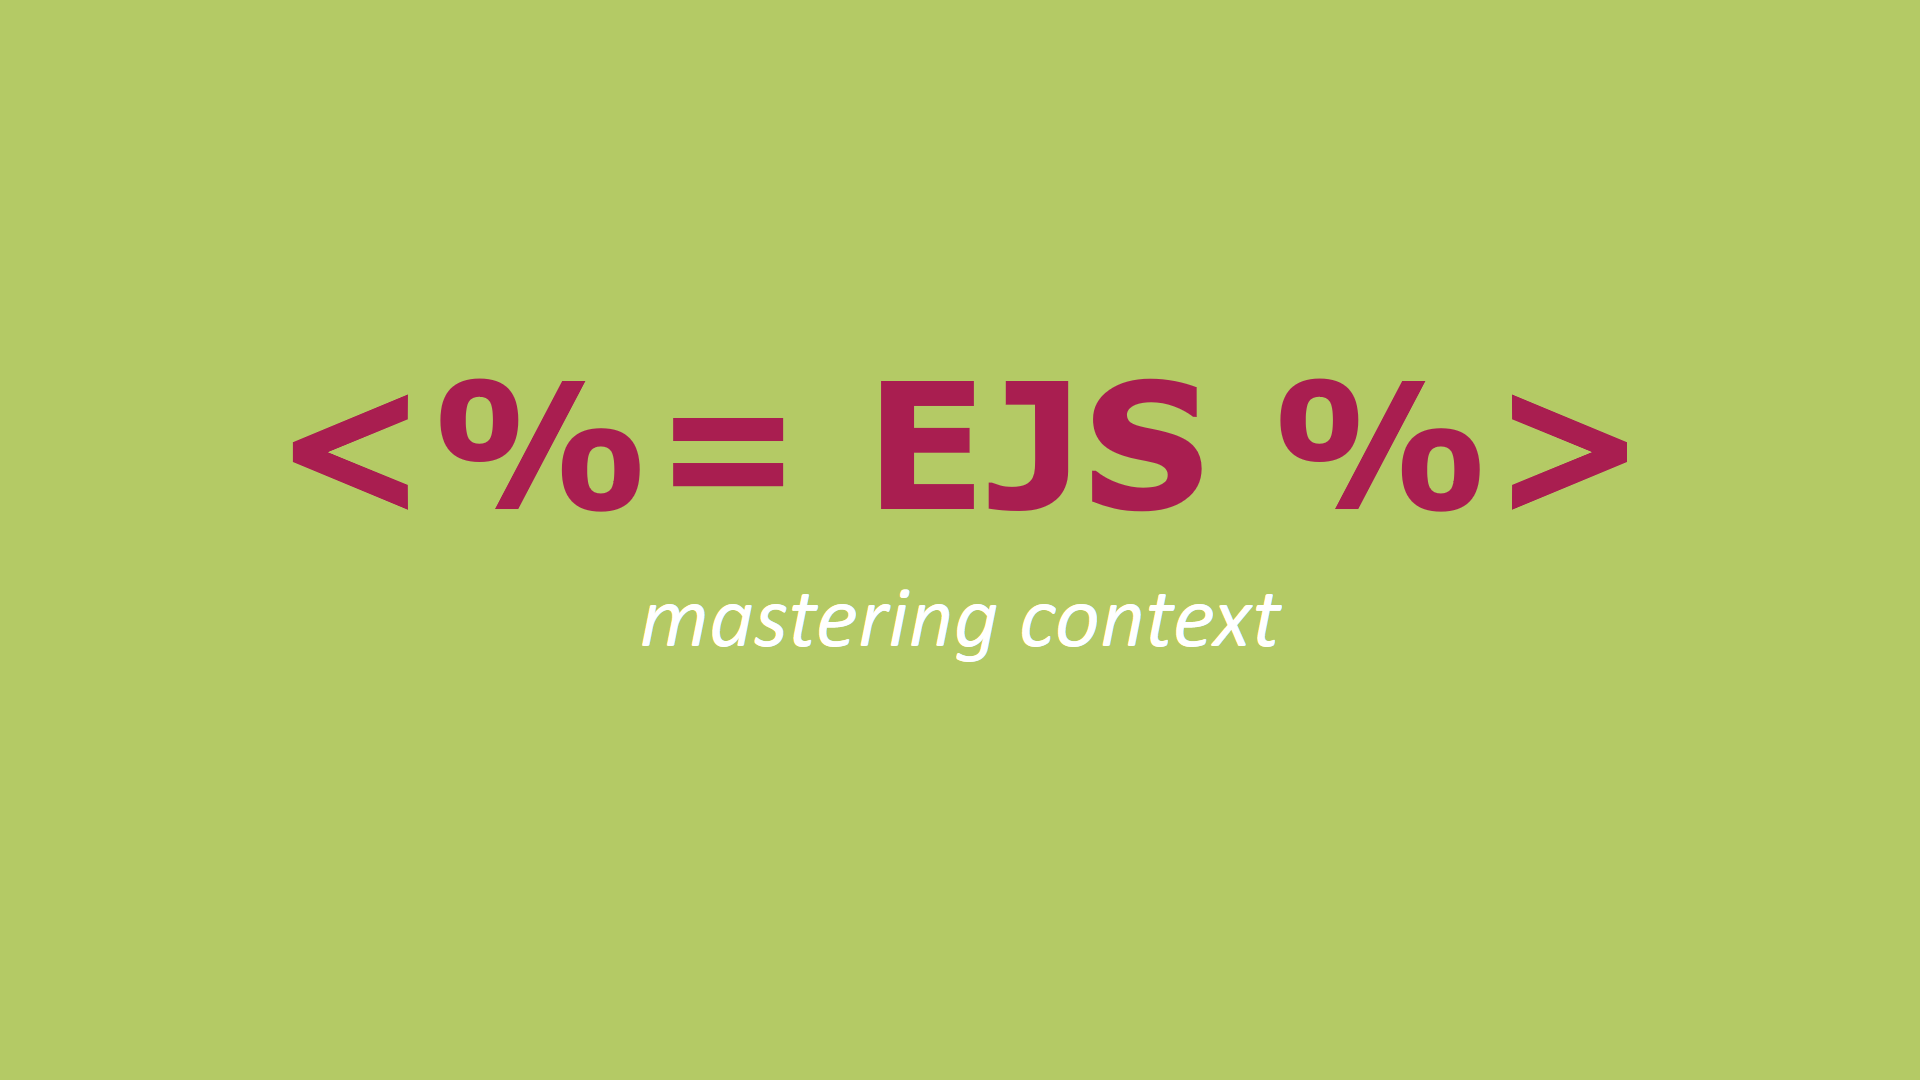
\includegraphics[width=4cm,height=3cm]{./figures/teklogos/ejs.png}
\caption{EJS.}
\end{figure}


\item {  \textbf{ Talend:} } [17]


 Est un éditeur de logiciel basé sur le langage JAVA spécialisé dans l'intégration de données.


\begin{figure}[H]
\center

\includegraphics[width=4cm,height=3cm]{./figures/teklogos/talend.png}
\caption{Talend.}
\end{figure}


\item {  \textbf{ Highcharts:} } [15]


L'outil de \guillemotleft{} reporting \guillemotright{} sur les pages web.


\begin{figure}[H]
\center

\includegraphics[width=4cm,height=3cm]{./figures/teklogos/highcharts.png}
\caption{Highcharts.}
\end{figure}


\end{itemize} 

\subsection{Mod\`{e}le du liason des donn\'{e}es }
L'architecture de notre application nous implique \`{a} cr\'{e}er un mod\`{e}le physique
des donn\'{e}es , et nous avons pas \'{e}t\'{e} besoin d'un model conceptuel logique
,puisque on a li\'{e}e directement les donn\'{e}es \`{a} l'application par le biais d'un
pilote de connexion et pas par un ORM , et ceci est le diagramme
Entit\'{e}s \textendash{}Relations de la base de donn\'{e}es qui est en interaction avec
l'application web .
Choix de la m\'{e}thodologie de conception :
La liaison par des ORM ,ou poss\'{e}de des avantages bienque des inconv\'{e}nient ,
parmi ses avantages :

\bigskip
\begin{itemize}
\item{\textbf{La portabilit\'{e} :}  ORM est utilis\'{e} pour que vous \'{e}criviez votre structure une
seule fois et la couche ORM g\'{e}rera l'instruction finale adapt\'{e}e au SGBD
configur\'{e}. C'est un excellent avantage, car une op\'{e}ration simple, telle que
limit, est ajout\'{e}e sous la forme "limit 0,100" \`{a} la fin de l'instruction select
dans MySQL, alors qu'elle est "select top 100 from table" dans MS SQL.}

\bigskip
\item{\textbf{Imbrication de donn\'{e}es:} en cas de relations, la couche ORM extraira
automatiquement les donn\'{e}es pour vous.}

\bigskip
\item{\textbf{Langage unique:} vous ne connaissez pas le langage SQL pour traiter la base
de donn\'{e}es uniquement avec votre langage de d\'{e}veloppement.
Ajouter revient \`{a} modifier: la plupart des couches ORM traitent l'ajout de
nouvelles donn\'{e}es (insertion SQL) et la mise \`{a} jour des donn\'{e}es (SQL
Update) de la m\^{e}me mani\`{e}re, ce qui facilite grandement l'\'{e}criture et la
maintenance du code.}

\item{\textbf{Imbrication de donn\'{e}es:} en cas de relations, la couche ORM extraira
automatiquement les donn\'{e}es pour vous.}

\end{itemize}

\bigskip

Et parmi les inconv\'{e}nients de l'ORM on trouve :



\bigskip

\begin{itemize}
\item{\textbf{ La complexit\'{e} des requ\^{e}tes : }certaines couches ORM ont des limitations, en
particulier lors de l'ex\'{e}cution de requ\^{e}tes. Vous serez donc parfois oblig\'{e}
d'\'{e}crire en SQL brut.}

\item{\textbf{Lenteur:}
 si vous comparez les performances entre l'\'{e}criture de SQL brut ou
l'utilisation d'ORM, vous trouverez le brut beaucoup plus rapidement car il
n'y a pas de couche de traduction.}

\item{\textbf{R\'{e}glage:} si vous connaissez bien le langage SQL et votre SGBD par d\'{e}faut,
vous pouvez utiliser vos connaissances pour acc\'{e}l\'{e}rer les requ\^{e}tes, mais ce
n'est pas la m\^{e}me chose avec ORM.}

\item{\textbf{Configuration:}
 si vous travaillez dans un projet Big Data et que vous n'\^{e}tes
pas satisfait de la performance, vous vous retrouverez en train d'\'{e}tudier la
couche ORM afin de pouvoir minimiser les occurrences du SGBD.}



\end{itemize}


\section{Conclusion}
Dans ce chapitre, nous avons vus les étapes analytiques dans laquelle nous avons recensé et
factorisé et les besoins des utilisateurs de l'application ainsi que l'architecture et les principaux
outils utilisés pour la construire . \newline
Dans le chapitre suivant nous entamons
le développement du premier release en suivant les lignes directrices que nous nous sommes
fixées.

